\documentclass[11pt,a4paper]{article}

\usepackage[utf8]{inputenc}
\usepackage[T1]{fontenc}
\usepackage[spanish, es-nodecimaldot]{babel}
\addto\captionsspanish{\renewcommand{\tablename}{Tabla}}
\usepackage{geometry}
\geometry{margin=2.5cm}
\usepackage{booktabs}
\usepackage{array}
\usepackage{hyperref}
\hypersetup{colorlinks=true, linkcolor=black, urlcolor=blue}
\usepackage{parskip}
\usepackage{listings}
\usepackage{xcolor}
\usepackage{enumitem}
\usepackage{graphicx}

\lstset{
  language=Java,
  basicstyle=\ttfamily\small,
  keywordstyle=\color{blue}\bfseries,
  commentstyle=\color{gray}\itshape,
  stringstyle=\color{teal},
  showstringspaces=false,
  breaklines=true,
  frame=single,
  framesep=4pt,
  xleftmargin=6pt,
  xrightmargin=6pt,
  aboveskip=6pt,
  belowskip=6pt,
}

\newcommand{\code}[1]{\texttt{#1}}
\newcommand{\file}[1]{\texttt{#1}}

\title{Informe de refactorización --- Fases~1, 2, 3 y~4\\
       \large \code{org.openmarkov.core} y módulos dependientes}
\author{Manuel Arias Calleja}
\date{Marzo de 2026}

\begin{document}

\maketitle
\tableofcontents
\newpage

% ===================================================================
\section*{Resumen ejecutivo}

Este informe documenta las modificaciones realizadas en las fases~1
(\emph{seguridad, concurrencia y excepciones}), 2 (\emph{encapsulación}),
3 (\emph{mejoras de API}) y~4 (\emph{eliminación de duplicación}) de la
campaña de refactorización sistemática de \code{org.openmarkov.core}.
El trabajo afectó a las cuatro clases de dominio más fundamentales del
módulo --- \code{ProbNet}, \code{Node}, \code{Variable} y \code{State} ---
y propagó los cambios de API a ocho módulos dependientes.

\begin{table}[!htbp]
\centering
\begin{tabular}{llc}
\toprule
\textbf{Fase} & \textbf{Área} & \textbf{Ficheros modificados} \\
\midrule
1.1 & Concurrencia: \code{PNESupport.listeners}       & 1 \\
1.2 & Concurrencia: \code{ProbNet.constantPotentials} & 1 \\
1.3 & Rollback en \code{ProbNet.setNetworkType()}     & 1 \\
1.4 & Documentación del constructor de \code{ProbNet} & 1 \\
1.5 & Concurrencia: \code{Node.potentials}            & 1 \\
2.1 & Encapsulación de campos en \code{Node}, \code{Variable}, \code{State} & 3 \\
2.2 & Encapsulación y corrección de bugs en \code{ProbNet} & 1 \\
2.3 & Actualización de módulos externos               & $\approx$30 \\
3.1 & Excepción incorrecta en \code{AugmentedProbTable} & 1 \\
3.2 & Validación de parámetros en \code{ProbNet.moveNode()} & 1 \\
3.3 & Casts sin \code{instanceof} en \code{ProbNet} y \code{Node} & 2 \\
3.4 & Descomposición de \code{Variable.modifyState()} & 1 \\
4.1 & Extracción de lógica de copia a \code{ProbNetCopier}        & 2 \\
4.2 & Unificación de variantes \code{getPotentials} con \code{Predicate} & 2 \\
4.3 & Creación de \code{UniformPotential} delegada en \code{PotentialOperations} & 1 \\
\bottomrule
\end{tabular}
\caption{Resumen de actividad por subpunto.}
\end{table}

% ===================================================================
\section{Fase 1 --- Seguridad, concurrencia y excepciones}

% -------------------------------------------------------------------
\subsection{Concurrencia en \code{PNESupport}: campo \code{listeners}
            (punto~1.1)}

\subsubsection*{Estado anterior}

\begin{lstlisting}
private HashSet<PNEditListener> listeners = new HashSet<>();
\end{lstlisting}

El campo era un \code{HashSet} mutable no sincronizado que se exponía
directamente a través del getter:

\begin{lstlisting}
public HashSet<PNEditListener> getListeners() {
    return listeners;
}
\end{lstlisting}

\subsubsection*{Riesgos}

\begin{enumerate}[label=(\alph*)]
  \item \textbf{\code{ConcurrentModificationException}.}
    Si un hilo itera el conjunto en \code{notifyListeners()} mientras
    otro hilo invoca \code{addListener()} o \code{removeListener()},
    el iterador de \code{HashSet} lanza \code{ConcurrentModification\-Exception}
    inmediatamente porque detecta la modificación estructural del conjunto
    durante la iteración. Este tipo de fallo es no determinista y difícil
    de reproducir en pruebas.

  \item \textbf{Exposición de la referencia interna.}
    Al devolver el propio \code{HashSet}, el código cliente podía añadir
    o eliminar listeners sin pasar por el contrato de \code{PNESupport},
    eludiendo cualquier lógica que se añadiese en el futuro en los métodos
    \code{addListener} y \code{removeListener}.

  \item \textbf{Reasignación directa del campo.}
    El método \code{setListeners()} reemplazaba la referencia del campo:
    si un hilo poseía una referencia al antiguo \code{HashSet}, seguiría
    usando el conjunto obsoleto; los nuevos eventos dejarían de llegarle.
\end{enumerate}

\subsubsection*{Solución}

\begin{lstlisting}
private final Set<PNEditListener> listeners =
        ConcurrentHashMap.newKeySet();
\end{lstlisting}

\begin{itemize}
  \item \code{ConcurrentHashMap.newKeySet()} produce un conjunto con la
    semántica de \code{Set} que soporta lecturas y escrituras concurrentes
    sin lanzar \code{ConcurrentModificationException} (los iteradores son
    \emph{weakly consistent}).
  \item El campo se declara \code{final}: su identidad no cambia, solo
    su contenido.
  \item \code{getListeners()} devuelve
    \code{Collections.unmodifiableSet(listeners)}: vista de solo lectura
    que impide modificaciones externas sin pasar por los métodos de la
    clase.
  \item \code{setListeners()} realiza \code{clear()} + \code{addAll()}
    sobre el mismo conjunto en lugar de reasignar el campo.
\end{itemize}

% -------------------------------------------------------------------
\subsection{Concurrencia en \code{ProbNet}: campo \code{constantPotentials}
            (punto~1.2)}

\subsubsection*{Estado anterior}

\begin{lstlisting}
private HashSet<Potential> constantPotentials = new HashSet<>();
\end{lstlisting}

\subsubsection*{Riesgos}

Idénticos al caso anterior: \code{HashSet} sin sincronización expuesto a
través de un getter que devuelve la referencia directa. La diferencia es
que \code{constantPotentials} se usa en operaciones de inferencia, que en
versiones futuras del motor pueden ejecutarse en hilos de trabajo separados.

\subsubsection*{Solución}

\begin{lstlisting}
private final Set<Potential> constantPotentials =
        ConcurrentHashMap.newKeySet();
\end{lstlisting}

\code{getConstantPotentials()} pasa a devolver
\code{Collections.unmodifiableSet(constantPotentials)}.

% -------------------------------------------------------------------
\subsection{Rollback en \code{ProbNet.setNetworkType()} (punto~1.3)}

\subsubsection*{Estado anterior}

\begin{lstlisting}
public void setNetworkType(NetworkType networkType) {
    NetworkType oldNetworkType = this.networkType;
    this.networkType = networkType;
    try {
        this.doEdit(new SetNetworkTypeEdit(this, networkType));
    } catch (Exception e) {
        throw new UnreachableException(e);
    }
}
\end{lstlisting}

La variable \code{oldNetworkType} se declaraba y asignaba pero nunca se
usaba para ningún propósito. En caso de que \code{doEdit} lanzase una
excepción (por ejemplo, porque la nueva restricción de tipo de red viola
alguna restricción de la estructura existente), el campo \code{this.networkType}
ya había sido modificado antes de que se detectase el error.

\subsubsection*{Riesgo: objeto en estado inconsistente}

Tras un fallo, \code{this.networkType} quedaría con el valor nuevo que no
pudo validarse, mientras que el grafo contenido en \code{this} no habría
cambiado para satisfacer las restricciones del nuevo tipo. Cualquier
operación posterior que consultase el tipo de red obtendría un valor que
no se corresponde con la estructura real del grafo.

\subsubsection*{Solución}

\begin{lstlisting}
public void setNetworkType(NetworkType networkType) {
    NetworkType oldNetworkType = this.networkType;
    this.networkType = networkType;
    try {
        this.doEdit(new SetNetworkTypeEdit(this, networkType));
    } catch (Exception e) {
        this.networkType = oldNetworkType;   // rollback
        throw new UnreachableException(e);
    }
}
\end{lstlisting}

Se añade la línea de rollback \code{this.networkType = oldNetworkType} en
el bloque \code{catch}, de modo que si la validación falla el objeto queda
exactamente como estaba antes de llamar al método.

% -------------------------------------------------------------------
\subsection{Documentación del constructor de \code{ProbNet} (punto~1.4)}

El constructor principal de \code{ProbNet} envuelve las posibles excepciones
de \code{doEdit} en \code{UnreachableException}. Se añadió Javadoc explicando
que se usa \code{ThrowableUtils.transferStackTrace} para preservar la cadena
de causa y el \emph{stack trace} original, evitando que la información de
diagnóstico se pierda en el envoltorio.

% -------------------------------------------------------------------
\subsection{Concurrencia en \code{Node}: campo \code{potentials}
            (punto~1.5)}

\subsubsection*{Estado anterior}

\begin{lstlisting}
protected List<Potential> potentials;
// inicializado en el constructor como:
this.potentials = new ArrayList<>();
\end{lstlisting}

Los métodos \code{setPotential()} y \code{setPotentials()} realizaban
operaciones compuestas sobre la lista:

\begin{lstlisting}
public void setPotentials(List<Potential> potentials) {
    this.potentials.clear();
    this.potentials.addAll(potentials);
}
\end{lstlisting}

\subsubsection*{Riesgos}

\begin{enumerate}[label=(\alph*)]
  \item \textbf{\code{ArrayList} no es hilo-seguro.}
    Lecturas concurrentes desde código de inferencia y escrituras desde
    el hilo de edición pueden provocar \code{ArrayIndexOutOfBoundsException}
    o devolver una lista parcialmente actualizada.

  \item \textbf{Operación compuesta no atómica.}
    Incluso usando \code{Collections.synchronizedList()}, la secuencia
    \code{clear()} + \code{addAll()} no sería atómica: entre ambas
    llamadas, otro hilo podría ver la lista vacía.
\end{enumerate}

\subsubsection*{Solución}

\begin{lstlisting}
this.potentials = Collections.synchronizedList(new ArrayList<>());
\end{lstlisting}

Las operaciones simples sobre la lista (lectura individual, iteración
en bloque propio del objeto) quedan protegidas. Para las operaciones
compuestas se añade un bloque \code{synchronized} explícito:

\begin{lstlisting}
public void setPotentials(List<Potential> potentials) {
    synchronized (this.potentials) {
        this.potentials.clear();
        this.potentials.addAll(potentials);
    }
}
\end{lstlisting}

% ===================================================================
\section{Fase 2 --- Encapsulación}

El objetivo de esta fase es eliminar los campos \code{public} y
\code{protected} de las clases de dominio fundamentales, sustituyéndolos
por campos \code{private} con métodos de acceso bien definidos. La
motivación general es triple:

\begin{enumerate}
  \item \textbf{Invariantes.} Los campos públicos pueden ser escritos
    desde cualquier punto del código sin ninguna validación, lo que hace
    imposible mantener invariantes de clase (por ejemplo, que el mapa de
    propiedades nunca sea \code{null}).
  \item \textbf{Defensibilidad ante cambios.} Un campo público es una
    API pública; cambiar su tipo o semántica futura requiere modificar
    todos los accesos dispersos por el código base. Un método accessor
    puede evolucionar internamente sin alterar la firma.
  \item \textbf{Copias defensivas.} Los arrays y colecciones expuestos
    directamente pueden ser modificados externamente, rompiendo el estado
    del objeto.
\end{enumerate}

% -------------------------------------------------------------------
\subsection{Campo \code{nodeType} de \code{Node} (punto~2.1)}

\subsubsection*{Estado anterior}

\begin{lstlisting}
protected NodeType nodeType;
\end{lstlisting}

\subsubsection*{Problema}

Al ser \code{protected}, las subclases y las clases del mismo paquete
podían escribir directamente sobre \code{nodeType}, eludiendo cualquier
control de acceso. Se encontraron accesos directos de escritura en
\code{ProbNet} (líneas~907 y~1230) y en \code{DecisionTreeNode}
(línea~174), todos ellos dentro del mismo proyecto.

\subsubsection*{Solución}

\begin{lstlisting}
private NodeType nodeType;
\end{lstlisting}

Todos los accesos directos se reemplazaron por llamadas a
\code{getNodeType()}.

% -------------------------------------------------------------------
\subsection{Campos \code{states} y \code{variableType} de \code{Variable}
            (punto~2.1)}

\subsubsection*{Estado anterior}

\begin{lstlisting}
protected State[] states;
protected VariableType variableType;
\end{lstlisting}

\subsubsection*{Problema con \code{states}}

Un array Java es mutable por referencia: si \code{getStates()} devuelve
\code{this.states}, el llamador puede escribir \code{states[i] = new State(...)}
y modificar el estado interno del objeto sin que este sea consciente. El
acceso \code{protected} además permitía a las subclases reasignar la
referencia completa.

\subsubsection*{Solución}

\begin{lstlisting}
private State[] states;

public State[] getStates() {
    return states.clone();   // copia defensiva
}

public void setStates(State[] states) {
    this.states = states.clone();   // copia defensiva
}
\end{lstlisting}

Tanto el getter como el setter realizan una copia defensiva
(\code{clone()}) para garantizar que el array interno no pueda ser
modificado externamente.

\code{variableType} se hace \code{private} sin necesidad de copia
defensiva porque \code{VariableType} es un \code{enum} (tipo por
valor).

% -------------------------------------------------------------------
\subsection{Campo \code{additionalProperties} en \code{ProbNet}, \code{Node},
            \code{Variable} y \code{State} (punto~2.2)}

\subsubsection*{Estado anterior}

Las cuatro clases tenían un campo de propiedades arbitrarias con
visibilidades inadecuadas:

\begin{center}
\begin{tabular}{lll}
\toprule
\textbf{Clase} & \textbf{Visibilidad anterior} & \textbf{Tipo anterior} \\
\midrule
\code{ProbNet}  & \code{public}    & \code{LinkedHashMap<String,String>} \\
\code{Node}     & \code{public}    & \code{LinkedHashMap<String,String>} \\
\code{Variable} & \code{protected} & \code{HashMap<String,String>} \\
\code{State}    & \code{public}    & \code{LinkedHashMap<String,String>} \\
\bottomrule
\end{tabular}
\end{center}

\subsubsection*{Riesgos}

\begin{enumerate}[label=(\alph*)]
  \item \textbf{Mutación directa.} Cualquier código podía llamar a
    \code{x.additionalProperties.put(k, v)}, \code{x.additional\-Properties.remove(k)}
    o incluso \code{x.additionalProperties = null}, rompiendo el invariante
    de que el mapa existe siempre.

  \item \textbf{Semántica de copia rota.} Dado que el campo era público,
    el código de copia lo asignaba directamente:
    \begin{lstlisting}
newNode.additionalProperties = CloneUtils.safeClone(this.additionalProperties);
    \end{lstlisting}
    Esto exige que quien hace la copia conozca el tipo concreto del campo
    (no la interfaz), e impide cambiar la implementación interna.
\end{enumerate}

\subsubsection*{Bugs descubiertos durante la encapsulación}

Al encapsular el campo se detectaron dos bugs en los métodos de copia de
\code{ProbNet}:

\paragraph{Bug en \code{ProbNet.auxCopy()} (línea~550).}

\begin{lstlisting}
// Codigo buggy:
newNode.additionalProperties = additionalProperties;
//               ^-- campo de ProbNet, no del nodo que se copia
\end{lstlisting}

El código asignaba el mapa de propiedades de la \emph{red} al nodo
recién creado, en lugar de copiar las propiedades del \emph{nodo} fuente.
Esto hacía que todos los nodos de la copia compartiesen el mismo mapa de
propiedades (el de la red), y que las propiedades específicas de cada nodo
se perdiesen completamente. Además, al compartir la referencia, cualquier
modificación a las propiedades de un nodo afectaría a todos los demás y a
la propia red.

\paragraph{Bug en \code{ProbNet.addShiftedNode()} (línea~1348).}

Idéntico al anterior: el código copiaba el mapa de propiedades de la
red en el nodo desplazado temporalmente, en lugar de copiar las
propiedades del nodo original.

\paragraph{Corrección.}

\begin{lstlisting}
// Codigo corregido (ambos metodos):
newNode.setAdditionalProperties(node.getAdditionalProperties());
\end{lstlisting}

\subsubsection*{Solución general}

Los cuatro campos se convierten a \code{private final Map<String,String>}
inicializado en la declaración (o en el constructor cuando procede).
Se añaden tres métodos en cada clase:

\begin{lstlisting}
/** Vista no modificable del mapa de propiedades adicionales. */
public Map<String, String> getAdditionalProperties() {
    return Collections.unmodifiableMap(additionalProperties);
}

/** Reemplaza todo el contenido del mapa. */
public void setAdditionalProperties(Map<String, String> properties) {
    additionalProperties.clear();
    additionalProperties.putAll(properties);
}

/** Inserta o actualiza una propiedad individual. */
public void putAdditionalProperty(String key, String value) {
    additionalProperties.put(key, value);
}
\end{lstlisting}

\paragraph{Diseño del getter.}
Devolver \code{Collections.unmodifiableMap()} en lugar de una copia tiene
coste cero y proporciona una vista en tiempo real del mapa que, sin embargo,
no puede ser modificada por el llamador. Esto es preferible a una copia
cuando el uso típico es solo de lectura (iterar propiedades al serializar
o mostrar).

\paragraph{Diseño del setter.}
En lugar de reasignar la referencia del campo (imposible al ser \code{final}),
se vacía el mapa existente y se vuelcan los nuevos pares. De este modo se
preserva la invariante de que el campo nunca es \code{null} y se mantiene
la identidad del mapa (sin invalidar vistas no modificables existentes).

\paragraph{Estandarización del nombre.}
Los métodos anteriores se llamaban \code{getOtherProperties()} y
\code{setOtherProperties()}, nombres inconsistentes con el nombre del
campo \code{additionalProperties}. Se han renombrado a
\code{getAdditionalProperties()} y \code{setAdditionalProperties()}
respectivamente.

% -------------------------------------------------------------------
\subsection{Actualización de módulos externos (punto~2.3)}

La encapsulación de los campos \code{additionalProperties} en las clases
de \code{core} rompió la compilación en ocho módulos dependientes.
Se actualizaron todos los accesos directos al campo aplicando las
siguientes transformaciones mecánicas:

\begin{center}
\begin{tabular}{ll}
\toprule
\textbf{Patrón antiguo} & \textbf{Patrón nuevo} \\
\midrule
\code{x.additionalProperties = m}             & \code{x.setAdditionalProperties(m)} \\
\code{x.additionalProperties.put(k,v)}        & \code{x.putAdditionalProperty(k,v)} \\
\code{x.additionalProperties.get(k)}          & \code{x.getAdditionalProperties().get(k)} \\
\code{x.additionalProperties.keySet()}        & \code{x.getAdditionalProperties().keySet()} \\
\code{x.additionalProperties.entrySet()}      & \code{x.getAdditionalProperties().entrySet()} \\
\code{x.getOtherProperties()}                 & \code{x.getAdditionalProperties()} \\
\code{x.setOtherProperties(m)}                & \code{x.setAdditionalProperties(m)} \\
\bottomrule
\end{tabular}
\end{center}

Los módulos afectados fueron:

\begin{itemize}
  \item \code{org.openmarkov.io}: \file{ElviraParser.java},
    \file{ElviraWriter.java}, \file{ElviraUtil.java},
    \file{PGMXReader\_0\_2.java}, \file{PGMXWriter\_0\_2.java}
    (con sus tests: \file{ElviraParserTest.java},
    \file{ElviraParserSVTest.java}).

  \item \code{org.openmarkov.io.database.excel}:
    \file{OldExcelDataBaseIO.java}, \file{CSVDataBaseIO.java},
    \file{ExcelDataBaseIO.java}.

  \item \code{org.openmarkov.io.database.weka}:
    \file{ArffParser.java}, \file{ArffDataBaseIO.java}.

  \item \code{org.openmarkov.io.database.elvira}:
    \file{ElviraDBParser.java}, \file{ElviraDataBaseIO.java}.

  \item \code{org.openmarkov.gui}:
    \file{PasteEdit.java}, \file{OtherPropertyEdit.java},
    \file{PrefixedOtherPropertiesTablePanel.java}.

  \item \code{org.openmarkov.learning.core}:
    \file{LearningManager.java} (tres líneas que leían el mapa
    mutable, añadían una clave y lo reasignaban se simplificaron
    a una única llamada \code{putAdditionalProperty("hasElviraProperties","yes")}).

  \item \code{org.openmarkov.integrationtests}:
    \file{Classificator.java} (accesos a
    \code{ProbNet.additionalProperties} y \code{State.additionalProperties}).
\end{itemize}

\paragraph{Caso especial: \code{ElviraWriter.generateElviraProperties()}.}

Este método obtenía una referencia directa al mapa de propiedades del nodo
y lo mutaba:

\begin{lstlisting}
// Codigo buggy:
Map<String, String> infoNode = node.additionalProperties;
// ... mutaciones sobre infoNode ...
\end{lstlisting}

Con el nuevo API, \code{getAdditionalProperties()} devuelve una vista no
modificable, por lo que la mutación directa lanzaría
\code{UnsupportedOperationException} en tiempo de ejecución. Se corrigió
copiando primero el mapa, aplicando las mutaciones sobre la copia y
finalmente persistiendo con \code{setAdditionalProperties()}:

\begin{lstlisting}
Map<String, String> infoNode = new LinkedHashMap<>(node.getAdditionalProperties());
// ... mutaciones sobre infoNode ...
node.setAdditionalProperties(infoNode);
\end{lstlisting}

\paragraph{Caso especial: \code{OtherPropertyEdit} en el módulo GUI.}

Este editor de propiedades utilizaba \code{LinkedHashMap} como tipo concreto
en su API interna (campos, parámetros y la llamada a \code{.clone()}).
Se migró a la interfaz \code{Map<String,String>} y se sustituyeron las
llamadas a \code{.clone()} por \code{new LinkedHashMap<>(...)}, que es
la forma canónica de copiar un mapa:

\begin{lstlisting}
// Antes:
this.newProperties = (LinkedHashMap<String,String>) this.oldProperties.clone();
// Despues:
this.newProperties = new LinkedHashMap<>(this.oldProperties);
\end{lstlisting}

% ===================================================================
\section{Fase 3 --- Mejoras de API}

El objetivo de esta fase es corregir puntos de la API interna de
\code{core} que presentan errores de contrato, ausencia de validación
o complejidad excesiva, sin modificar las firmas públicas visibles
desde los módulos dependientes.

% -------------------------------------------------------------------
\subsection{Excepción semánticamente incorrecta en
            \code{AugmentedProbTable} (punto~3.1)}

\subsubsection*{Estado anterior}

\begin{lstlisting}
} catch (NegativeArraySizeException e) {
    throw new OutOfMemoryError(e.getMessage());
}
\end{lstlisting}

\subsubsection*{Problemas}

\begin{enumerate}[label=(\alph*)]
  \item \textbf{Causa perdida.} \code{OutOfMemoryError} no expone un
    constructor \code{(Throwable cause)}, por lo que la excepción
    original --- incluyendo su \emph{stack trace} y mensaje --- desaparece
    por completo. Cualquier herramienta de diagnóstico o registro de errores
    verá solo el \code{OutOfMemoryError} con el mensaje copiado como cadena,
    sin poder navegar hasta el origen real del fallo.

  \item \textbf{Tipo semánticamente incorrecto.} \code{OutOfMemoryError}
    indica que la JVM no puede asignar más memoria del \emph{heap}.
    Un array de tamaño negativo es una violación de precondición
    (el argumento \code{tableSize} tiene un valor ilegal), no un
    agotamiento de recursos. Lanzar \code{OutOfMemoryError} induce a
    confusión: los sistemas de monitorización tratarán el evento como
    un fallo de memoria y no como un error de programación.
\end{enumerate}

\subsubsection*{Solución}

\begin{lstlisting}
} catch (NegativeArraySizeException e) {
    throw new IllegalArgumentException(
            "Negative table size: " + tableSize, e);
}
\end{lstlisting}

\code{IllegalArgumentException} es el tipo estándar de Java para
precondiciones violadas. El segundo argumento preserva la causa original
en la cadena de excepciones.

% -------------------------------------------------------------------
\subsection{Validación de parámetros en \code{ProbNet.moveNode()}
            (punto~3.2)}

\subsubsection*{Estado anterior}

\begin{lstlisting}
public void moveNode(List<String> namesNode,
                     List<Point2D.Double> newPositions) {
    Node node;
    int i = 0;
    for (String name : namesNode) {
        node = getNode(name);
        node.setCoordinateX(newPositions.get(i).getX());
        node.setCoordinateY(newPositions.get(i).getY());
        i++;
    }
}
\end{lstlisting}

\subsubsection*{Problema}

El método acepta dos listas que deben tener exactamente el mismo
tamaño: la lista de nombres de nodo y la lista de posiciones nuevas.
Si el llamador pasa listas de tamaños distintos, el bucle agota la
lista más corta sin error (si \code{namesNode} es más corta) o lanza
\code{IndexOutOfBoundsException} en \code{newPositions.get(i)} cuando
\code{namesNode} es más larga. En ambos casos la red queda en un
estado parcialmente actualizado sin ningún mensaje descriptivo que
indique el origen del problema.

\subsubsection*{Solución}

\begin{lstlisting}
public void moveNode(List<String> namesNode,
                     List<Point2D.Double> newPositions) {
    if (namesNode.size() != newPositions.size()) {
        throw new IllegalArgumentException(
                "namesNode and newPositions must have the same size: "
                + namesNode.size() + " vs " + newPositions.size());
    }
    int i = 0;
    for (String name : namesNode) {
        Node node = getNode(name);
        node.setCoordinateX(newPositions.get(i).getX());
        node.setCoordinateY(newPositions.get(i).getY());
        i++;
    }
}
\end{lstlisting}

La validación al inicio del método es la forma canónica de expresar
precondiciones en Java: falla rápido, con un mensaje que identifica
el tamaño real de cada lista.

% -------------------------------------------------------------------
\subsection{Casts sin \code{instanceof} previo (punto~3.3)}

Se corrigieron dos \emph{bare casts} en los que el compilador no
puede garantizar el tipo en tiempo de compilación y un fallo
producía \code{ClassCastException} sin contexto.

\paragraph{\code{ProbNet.buildMarkovDecisionNetwork()} --- cast a \code{TablePotential}.}

\begin{lstlisting}
// Antes:
// TODO - Change constant potentials (Potential vs TablePotential)
this.constantPotentials.add((TablePotential) potential);

// Despues:
if (!(potential instanceof TablePotential tablePotential)) {
    throw new IllegalArgumentException(
            "Constant potential must be a TablePotential, got: "
            + potential.getClass().getName());
}
this.constantPotentials.add(tablePotential);
\end{lstlisting}

El TODO preexistente reconocía la deuda técnica de que
\code{constantPotentials} almacena \code{TablePotential} aunque el
campo que lo alimenta es de tipo \code{Potential}. Con el
\emph{pattern matching} se mantiene el comportamiento de fallo ante
tipos inesperados pero con un mensaje que identifica la clase recibida.

\paragraph{\code{Node.absorbNodeConsistently()} --- cast al resultado de \code{maximize()}.}

\begin{lstlisting}
// Antes:
TablePotential maximizedPotential =
    (TablePotential) DiscretePotentialOperations
                         .maximize(utilityPotential, absorbedVariable)[0];

// Despues:
// maximize()[0] is always a TablePotential per its contract
Object[] maximizeResult = DiscretePotentialOperations
        .maximize(utilityPotential, absorbedVariable);
if (!(maximizeResult[0] instanceof TablePotential maximizedPotential)) {
    throw new IllegalStateException(
            "maximize() expected to return a TablePotential at index 0, got: "
            + maximizeResult[0].getClass().getName());
}
\end{lstlisting}

\code{DiscretePotentialOperations.maximize(Potential, Variable)} devuelve
\code{Object[]} (diseño heredado), donde el elemento~0 es siempre un
\code{TablePotential} según el contrato del método. El \emph{pattern
matching} documenta este supuesto y lo convierte en un fallo explícito
si alguna futura modificación de \code{maximize()} lo rompiese, en lugar
de propagar un \code{ClassCastException} difícil de rastrear.

% -------------------------------------------------------------------
\subsection{Descomposición de \code{Variable.modifyState()} (punto~3.4)}

\subsubsection*{Estado anterior}

\code{Variable.modifyState()} era un método de 134~líneas con un
\code{switch} de cinco casos (ADD, REMOVE, DOWN, UP, RENAME), cada
uno con su propia lógica de manipulación del array de estados y del
\code{PartitionedInterval}. El único caller externo es
\code{NodeStateEdit.executeEdit()}.

\subsubsection*{Problema}

Un método de 134~líneas con cinco responsabilidades distintas viola
el principio de responsabilidad única. El código comparte variables
locales entre casos (\code{selectedStateIndex}, \code{oldStates},
\code{newState}) aunque cada caso usa un subconjunto diferente de
ellas, lo que dificulta entender qué datos son relevantes para cada
acción.

\subsubsection*{Solución}

\code{modifyState()} se reduce a un despachador de 12~líneas que
delega cada caso en un método privado:

\begin{lstlisting}
public void modifyState(Node node, StateAction stateAction,
                        int stateIndex, String newName) {
    int selectedStateIndex = stateAction != StateAction.ADD
            ? getNumStates() - (stateIndex + 1) : 0;
    switch (stateAction) {
        case ADD    -> addStateAt(node, stateIndex, newName);
        case REMOVE -> removeStateAt(node, selectedStateIndex);
        case DOWN   -> moveStateDown(node, selectedStateIndex);
        case UP     -> moveStateUp(node, selectedStateIndex);
        case RENAME -> renameState(selectedStateIndex, newName);
    }
}
\end{lstlisting}

Los cinco métodos privados extraídos son:

\begin{itemize}
  \item \code{addStateAt(Node, int, String)} --- inserta el nuevo
    estado en la posición indicada, actualiza el potencial y, si la
    variable es DISCRETIZED, recalcula el \code{PartitionedInterval}.
  \item \code{removeStateAt(Node, int)} --- elimina el estado en
    la posición inversa, actualiza el potencial y, si la variable es
    NUMERIC o DISCRETIZED, elimina el límite correspondiente del
    intervalo de partición.
  \item \code{moveStateDown(Node, int)} / \code{moveStateUp(Node, int)}
    --- intercambian dos estados adyacentes y reordenan los potenciales
    del nodo y sus hijos.
  \item \code{renameState(int, String)} --- renombra el objeto
    \code{State} en el índice indicado; como \code{getStates()} devuelve
    un clon del array pero los objetos \code{State} son referencias
    compartidas, la mutación actúa sobre el estado interno.
\end{itemize}

La firma pública de \code{modifyState()} no cambia; los callers
existentes no se ven afectados.

% ===================================================================
\section{Fase 4 --- Eliminación de duplicación}

El objetivo de esta fase es eliminar lógica repetida en las clases de
dominio de \code{core}, extrayendo el código común a métodos o clases
auxiliares bien nombrados. Las figuras~\ref{fig:fase4-antes}
y~\ref{fig:fase4-despues} muestran únicamente los métodos afectados,
antes y después de la refactorización.

\begin{figure}[!htbp]
  \centering
  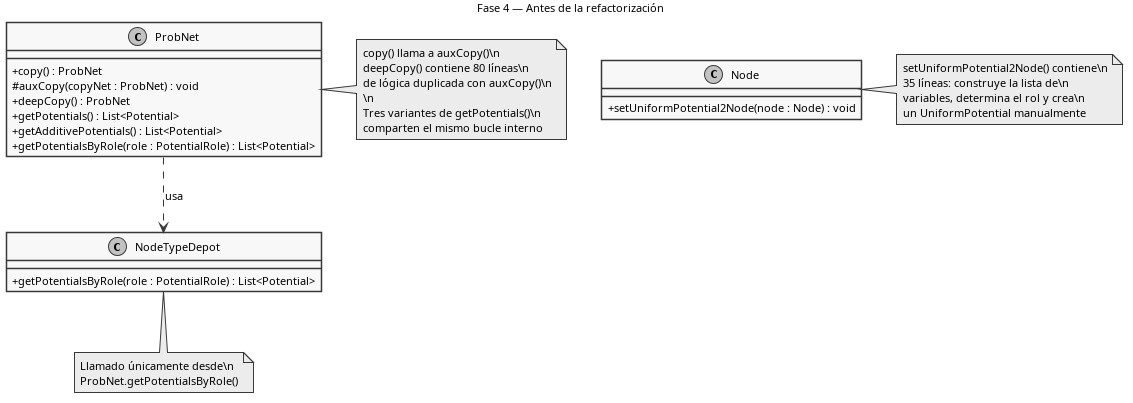
\includegraphics[width=0.82\textwidth]{fase4-antes.png}
  \caption{Diagrama de clases --- estado antes de la Fase~4.}
  \label{fig:fase4-antes}
\end{figure}

\begin{figure}[!htbp]
  \centering
  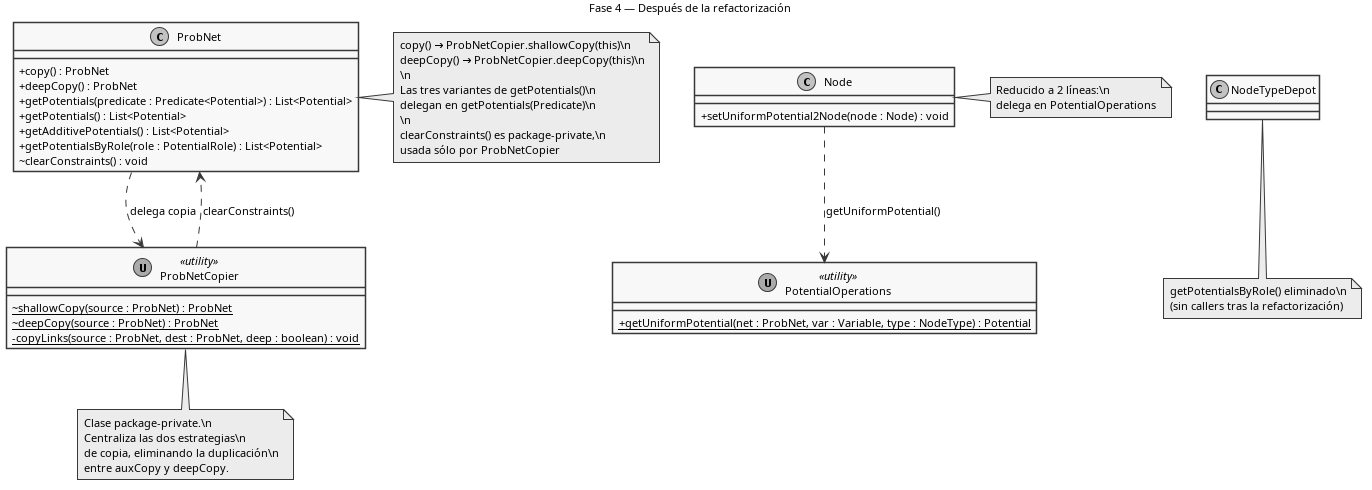
\includegraphics[width=0.92\textwidth]{fase4-despues.png}
  \caption{Diagrama de clases --- estado después de la Fase~4.}
  \label{fig:fase4-despues}
\end{figure}

% -------------------------------------------------------------------
\subsection{Unificación de la lógica de copia en \code{ProbNetCopier}
            (punto~4.1)}

\subsubsection*{Estado anterior}

\code{ProbNet} contenía dos métodos de copia con estructuras casi idénticas:

\begin{lstlisting}
// Copia superficial
protected ProbNet auxCopy(ProbNet copyNet) { ... }  // ~75 lineas
public ProbNet copy() {
    return auxCopy(new ProbNet(this.networkType));
}

// Copia profunda
public ProbNet deepCopy() { ... }  // ~80 lineas
\end{lstlisting}

Ambos métodos compartían el mismo esqueleto: copiar nombre, restricciones,
nodos, enlaces, listeners y propiedades adicionales, diferenciándose solo
en si los objetos (potenciales, nodos, intervalos) se compartían o se
clonaban. El bloque de copia de enlaces en particular era casi idéntico
línea a línea.

\subsubsection*{Riesgos}

\begin{enumerate}[label=(\alph*)]
  \item \textbf{Evolución divergente.} Cualquier corrección en la lógica
    de copia de enlaces (por ejemplo, añadir un nuevo campo a \code{Link})
    requería modificar ambos métodos de forma independiente, con riesgo de
    olvidar uno de ellos.
  \item \textbf{Visibilidad \code{protected} de \code{auxCopy}.} Al ser
    \code{protected}, el método formaba parte de la API de subclases aunque
    ninguna subclase de producción lo sobrescribía.
\end{enumerate}

\subsubsection*{Solución}

Se crea la clase de utilidad \code{ProbNetCopier} (misma package, acceso
package-private) con dos métodos estáticos:

\begin{lstlisting}
final class ProbNetCopier {
    static ProbNet shallowCopy(ProbNet source) { ... }
    static ProbNet deepCopy(ProbNet source) { ... }
    private static void copyLinks(ProbNet source, ProbNet dest,
                                  boolean deep) { ... }
}
\end{lstlisting}

El método privado \code{copyLinks} captura el único bucle que se repetía
en ambas copias, parametrizando la profundidad mediante un booleano.
\code{ProbNet} se reduce a delegaciones de una línea:

\begin{lstlisting}
public ProbNet copy() {
    return ProbNetCopier.shallowCopy(this);
}

public ProbNet deepCopy() {
    return ProbNetCopier.deepCopy(this);
}
\end{lstlisting}

Se añade además el método package-private \code{ProbNet.clearConstraints()}
para que \code{ProbNetCopier.deepCopy} pueda resetear el conjunto de
restricciones sin acceder al campo privado directamente.

% -------------------------------------------------------------------
\subsection{Unificación de variantes \code{getPotentials} con \code{Predicate}
            (punto~4.2)}

\subsubsection*{Estado anterior}

\code{ProbNet} y \code{NodeTypeDepot} contenían variantes del mismo bucle
``iterar todos los nodos, filtrar sus potenciales y añadirlos a una lista'':

\begin{lstlisting}
// Variante 1 - todos los potenciales no nulos
public List<Potential> getPotentials() {
    List<Potential> potentials = new ArrayList<>();
    for (Node node : getNodes()) {
        for (Potential p : node.getPotentials()) {
            if (p != null) potentials.add(p);
        }
    }
    for (Potential p : constantPotentials) {
        if (p != null) potentials.add(p);
    }
    return potentials;
}

// Variante 2 - solo los aditivos
public List<Potential> getAdditivePotentials() {
    List<Potential> potentials = new ArrayList<>();
    for (Node node : getNodes()) {
        for (Potential p : node.getPotentials()) {
            if (p != null && p.isAdditive()) potentials.add(p);
        }
    }
    // idem para constantPotentials...
}

// Variante 3 - por rol (en ProbNet, delegaba a NodeTypeDepot)
public List<Potential> getPotentialsByRole(PotentialRole role) {
    List<Potential> potentials = nodeDepot.getPotentialsByRole(role);
    for (Potential p : constantPotentials) {
        if (p.getPotentialRole() == role) potentials.add(p);
    }
    return potentials;
}
\end{lstlisting}

\subsubsection*{Solución}

Se añade un método base parametrizado con \code{Predicate<Potential>}:

\begin{lstlisting}
public List<Potential> getPotentials(Predicate<Potential> predicate) {
    List<Potential> potentials = new ArrayList<>();
    for (Node node : getNodes()) {
        for (Potential p : node.getPotentials()) {
            if (p != null && predicate.test(p)) potentials.add(p);
        }
    }
    for (Potential p : constantPotentials) {
        if (p != null && predicate.test(p)) potentials.add(p);
    }
    return potentials;
}
\end{lstlisting}

Las tres variantes se reducen a delegaciones de una línea:

\begin{lstlisting}
public List<Potential> getPotentials() {
    return getPotentials(p -> true);
}

public List<Potential> getAdditivePotentials() {
    return getPotentials(Potential::isAdditive);
}

public List<Potential> getPotentialsByRole(PotentialRole role) {
    return getPotentials(p -> p.getPotentialRole() == role);
}
\end{lstlisting}

El método \code{getPotentialsByRole} de \code{NodeTypeDepot} queda sin
callers y se elimina.

% -------------------------------------------------------------------
\subsection{Creación de \code{UniformPotential} delegada en
            \code{PotentialOperations} (punto~4.3)}

\subsubsection*{Estado anterior}

\code{Node.setUniformPotential2Node()} construía manualmente la lista de
variables (nodo + padres) y creaba un \code{UniformPotential}, lógica
que \code{PotentialOperations.getUniformPotential()} ya encapsulaba:

\begin{lstlisting}
public void setUniformPotential2Node(Node node) {
    List<Variable> variables = new ArrayList<>();
    PotentialRole role = node.getPotentials().getFirst().getPotentialRole();
    Variable thisVariable = node.getPotentials().getFirst().getVariable(0);
    variables.add(thisVariable);
    int numOfCellsInTable = thisVariable.getNumStates();
    double initialValue = Util.round(1.0 / numOfCellsInTable, "0.01");
    for (Node parent : node.getParents()) {
        variables.add(parent.getVariable());
        numOfCellsInTable *= parent.getVariable().getNumStates();
    }
    // TODO: This array is never used. Why is it created then?
    double[] table = new double[numOfCellsInTable];
    for (int i = 0; i < numOfCellsInTable; i++) table[i] = initialValue;

    UniformPotential uniformPotential = new UniformPotential(variables, role);
    node.setPotentials(new ArrayList<>(List.of(uniformPotential)));
}
\end{lstlisting}

El array \code{table} tiene incluso un TODO que reconoce que no se usa.

\subsubsection*{Solución}

Se sustituye el cuerpo completo por una delegación de dos líneas:

\begin{lstlisting}
public void setUniformPotential2Node(Node node) {
    Potential uniformPotential = PotentialOperations.getUniformPotential(
            node.getProbNet(), node.getVariable(), node.getNodeType());
    node.setPotentials(new ArrayList<>(List.of(uniformPotential)));
}
\end{lstlisting}

El array muerto desaparece junto con toda la construcción manual de la
lista de variables.

% ===================================================================
\section{Tabla resumen de cambios}

\begin{table}[!htbp]
\centering
\begin{tabular}{p{4.5cm} p{3.5cm} p{6cm}}
\toprule
\textbf{Clase / fichero} & \textbf{Campo / método} & \textbf{Cambio} \\
\midrule
\code{PNESupport}
  & \code{listeners}
  & \code{HashSet} → \code{ConcurrentHashMap.newKeySet()}; \code{final}; getter retorna vista no modificable \\
\addlinespace
\code{ProbNet}
  & \code{constantPotentials}
  & \code{HashSet} → \code{ConcurrentHashMap.newKeySet()}; \code{final}; getter retorna vista no modificable \\
\addlinespace
\code{ProbNet}
  & \code{setNetworkType()}
  & Añadido rollback \code{this.networkType = oldNetworkType} en bloque \code{catch} \\
\addlinespace
\code{Node}
  & \code{potentials}
  & \code{ArrayList} → \code{Collections.synchronizedList}; operaciones compuestas con \code{synchronized} \\
\addlinespace
\code{Node}
  & \code{nodeType}
  & \code{protected} → \code{private}; accesos directos sustituidos por \code{getNodeType()} \\
\addlinespace
\code{Node}
  & \code{additionalProperties}
  & \code{public LinkedHashMap} → \code{private final Map}; API: \code{getAdditionalProperties()}, \code{setAdditionalProperties()}, \code{putAdditionalProperty()} \\
\addlinespace
\code{Variable}
  & \code{states}
  & \code{protected State[]} → \code{private State[]}; getter y setter con \code{clone()} defensivo \\
\addlinespace
\code{Variable}
  & \code{variableType}
  & \code{protected} → \code{private} \\
\addlinespace
\code{Variable}
  & \code{additionalProperties}
  & \code{protected HashMap} → \code{private Map}; misma API que \code{Node} \\
\addlinespace
\code{State}
  & \code{additionalProperties}
  & \code{public LinkedHashMap} → \code{private final Map}; misma API que \code{Node} \\
\addlinespace
\code{ProbNet}
  & \code{additionalProperties}
  & \code{public LinkedHashMap} → \code{private final Map}; misma API que \code{Node} \\
\addlinespace
\code{ProbNet.auxCopy()}
  & línea~550
  & \textbf{Bug}: se copiaba el mapa de la red al nodo en lugar del mapa del nodo \\
\addlinespace
\code{ProbNet.addShiftedNode()}
  & línea~1348
  & \textbf{Bug}: ídem al anterior \\
\addlinespace
\code{ProbNet}
  & \code{copy()}, \code{deepCopy()}
  & Delegan en nueva clase \code{ProbNetCopier}; eliminado \code{auxCopy()} \\
\addlinespace
\code{ProbNetCopier} \emph{(nueva)}
  & \code{shallowCopy()}, \code{deepCopy()}, \code{copyLinks()}
  & Centraliza las dos estrategias de copia; \code{copyLinks} comparte el bucle de enlaces \\
\addlinespace
\code{ProbNet}
  & \code{getPotentials(Predicate)}
  & Nuevo método base; \code{getPotentials()}, \code{getAdditivePotentials()} y \code{getPotentialsByRole()} delegan en él \\
\addlinespace
\code{NodeTypeDepot}
  & \code{getPotentialsByRole()}
  & Eliminado (sin callers tras el punto~4.2) \\
\addlinespace
\code{Node}
  & \code{setUniformPotential2Node()}
  & Simplificado a 2~líneas usando \code{PotentialOperations.getUniformPotential()}; eliminado array \code{table} muerto \\
\bottomrule
\end{tabular}
\caption{Tabla resumen de todos los cambios realizados.}
\end{table}

% ===================================================================
\section{Conclusiones}

Las fases~1 y~2 de la refactorización eliminaron un conjunto de
vulnerabilidades estructurales presentes en el corazón del modelo de dominio:

\begin{itemize}
  \item \textbf{Dos bugs de copia} en \code{ProbNet} que hacían que los nodos
    copiados heredasen propiedades incorrectas (las de la red en lugar de
    las suyas propias), con posibilidad de interferencia entre nodos al
    compartir la misma referencia de mapa.

  \item \textbf{Un bug de estado inconsistente} en \code{setNetworkType()} que
    dejaba el objeto en un estado inválido tras un fallo de validación.

  \item \textbf{Tres puntos de carrera de datos} (\emph{data race}) en
    colecciones no sincronizadas accesibles concurrentemente.

  \item \textbf{Múltiples violaciones de encapsulación} que permitían a
    código externo modificar el estado interno de las clases de dominio
    sin pasar por ninguna validación.
\end{itemize}

La fase~3 corrigió errores de contrato en la API interna: excepción
semánticamente incorrecta, ausencia de validación de parámetros y casts
sin comprobación de tipo previa.

La fase~4 ha reducido la duplicación estructural en \code{ProbNet} y
\code{Node}:

\begin{itemize}
  \item \textbf{\code{ProbNetCopier}} centraliza las dos estrategias de copia
    de red (superficial y profunda) que antes convivían como métodos
    paralelos en \code{ProbNet}, extrayendo el bucle de copia de enlaces
    como método privado compartido.

  \item \textbf{\code{getPotentials(Predicate)}} elimina tres variantes
    del mismo bucle de recolección de potenciales, permitiendo expresar
    cualquier filtro futuro en una sola línea.

  \item \textbf{\code{Node.setUniformPotential2Node()}} delega en
    \code{PotentialOperations.getUniformPotential()}, eliminando la
    duplicación con \code{Variable.setUniformPotential()} y borrando
    un array temporal que el propio código reconocía como innecesario.
\end{itemize}

El coste acumulado de las cuatro fases es la actualización de
$\approx$50~puntos de uso en ocho módulos externos (fases~1--3) y la
creación de un fichero nuevo (\code{ProbNetCopier.java}) junto con la
eliminación de $\approx$160~líneas de código duplicado (fase~4).

\end{document}
